%%%%% START PREAMBLE HEADER %%%%%

%%% START REQUIRED PACKAGES %%%

\documentclass[twocolumn]{article}
\usepackage[a4paper, total={7.25in, 9.5in}]{geometry} 
\usepackage{multirow}
\usepackage{multicol}
\usepackage{lipsum}
\usepackage{hyperref}
\usepackage{listings}
\usepackage{graphicx}
\usepackage{import}
\usepackage{caption}
\usepackage[table,xcdraw]{xcolor}
\usepackage[export]{adjustbox}
%\usepackage[superscript,biblabel]{cite}
\usepackage{amsmath}
\hypersetup{colorlinks=true,linkcolor=blue,filecolor=magenta,urlcolor=cyan,citecolor=blue}

%%% END REQUIRED PACKAGES %%%                


%%% START NEW COMMANDS new (shortcut) %%%

% This is a paragraph with normal font
\newcommand{\np}[1]{\paragraph*{\normalfont{#1}}}
% This is a text with a color
\newcommand{\ct}[2]{\textcolor{#1}{#2}}
% This is a bold text 
\newcommand{\bt}[1]{\textbf{#1}}
% This is an italic text 
\newcommand{\et}[1]{\emph{#1}}
% This is an underline text 
\newcommand{\ut}[1]{\underline{#1}}
% This is a newline shortcut
\newcommand{\n}{\\}
% This is a numbered equation with break line shortcut
\newcommand{\necbreak}[1]{\begin{equation}\begin{aligned}#1\end{aligned}\end{equation}}
% This is a numbered equation with break line shortcut
\newcommand{\nec}[1]{\begin{equation}#1\end{equation}}
% This is an equation shortcut
\newcommand{\ec}[1]{\begin{center} $#1$ \end{center}}
% Table title with bold text and correct space%
\newcommand{\titleTable}[2]{\np{\bt{Table #1} #2}}% Graph title with bold text and correct space%
\newcommand{\titleGraph}[2]{\np{\bt{Graph #1} #2}}
% Table body with border %
\newcommand{\bodyTable}[2]{\begin{center} \begin{tabular}{|#1|} \hline #2 \hline \end{tabular} \end{center} }
%%% END NEW COMMANDS (shortcuts) %%%


%%% START TITLE SETTINGS %%%
\title{\bt{Practice \# 5 Battle of speed SET vs HAT, hydrogen abstraction of phenol with hydroperoxyl radical.}}
\author{Pérez Alvarado Luis Raymundo, School of Chemistry, UNAM}
\date{22/01/2021}
%%% END TITLE SETTINGS %%%

%%%%% END PREAMBLE HEADER %%%%%

%%%%%%%%%%%%%%%% START DOCUMENT %%%%%%%%%%%%%%%%
\begin{document}

    %%% THIS CONTENT IS IN ONE COLUMN (START) %%%
    \twocolumn[
        \begin{@twocolumnfalse}

            %% CREATE A TITLE (START) %%
            \maketitle
            %% CREATE A TITLE (END) %%

            %% CREATE A ABSTRACT (START,MAX 250 CHARACTERS) %%
            \begin{abstract}
                \item This report studied and compared two mechanisms for the abstraction of hydrogen from phenol with hydroperoxyl radical HAT and SET, with a normal procedure we calculate the transition state and $\Delta G^{\ddagger}$ for HAT, in the case of SET we calculated $\Delta G^{\ddagger}$ indirectly using the Marcus theory, and calculated the rate constant for each one, considered a fisiological pH to know the fraction mol of phenol and phenoxide in solution, and was determined that SET is the mechanism predominant for the abstraction of hydrogen via SPLET.
                \item \bt{Keywords:}\em{ Hydrogen abstraction, SET, HAT, Marcus theory.}
            \end{abstract}
            %% CREATE A ABSTRACT (END) %%
    
        \end{@twocolumnfalse}
    ]
    %%% THIS CONTENT IS IN ONE COLUMN (END) %%%

    %%% THIS CONTENT IS IN TWO COLUMN (START) %%%

    %% START SECTION %%

    % SECTION TITLE %
    \section{Introduction \small{$\cite{ania}\cite{vargas}$} }

    \np{The reaction mechanism antioxidants such as phenolic compounds can be divide into two groups in mechanisms of one step or more than one.}

    \subsection*{Single Step Mechanisms}

    \subsubsection*{Radical Adduct Formation (RAF)}

    \np{This reaction consists in the formation of an adduct radical, this usually is carotenoids, where the radical is stabilized by the delocalization of electron through the unsaturated long-chain and rings.}

    \nec{H-R + \cdot OOH \rightarrow [H-R-OOH]\cdot \label{1}}

    \subsubsection*{Single Electron Transfer (SET)}

    \np{Consist of the transference of one electron from the antioxidant to radical which converts into an anion with low reactivity than radical.}
    
    \np{This reaction can be with the antioxidant \eqref{2} or the anion of the antioxidant \eqref{3}.}

    \nec{H-R + \cdot OOH \rightarrow H-R\cdot + HOO^- \label{2}}

    \nec{R^- + \cdot OOH \rightarrow R\cdot + HOO^- \label{3}}

    \subsubsection*{Hydrogen Atom Transfer (HAT)}

    \np{This is the transfer of hydrogen atom from antioxidant to the radical a making it into a neutral molecule and forming a stable radical with the antioxidant.}

    \nec{R-H + \cdot OOH \rightarrow R\cdot + HOOH \label{4}}

    \subsubsection*{Proton Coupled Electron Transfer (PCET)}

    \np{The equation \eqref{4} is the same equation with PCET with the difference that this mechanism has a parallel step transferring a proton and electron and the same time.}

    \subsection*{Multiple Step Mechanisms}

    \subsubsection*{Sequential Proton Loss Electron Transfer (SPLET)}

    \np{This reaction consist in two step with the first is the deprotonation of the antioxidant by solvent \eqref{5} and SET reaction \eqref{3}}

    \nec{R-H + H_2O \rightarrow R^- + [H_3O2]^+ \label{5}}

    \np{HAT mechanisms can be described and get the $\Delta G^\dagger$ but in the case of SET mechanism can not calculate directly, the reason for this does not exist the transition state.}

    \subsection*{Marcus Theory \small{$\cite{web:marcus}$}}

    \np{The free energy of electron transfer is described in \eqref{6}.}

    \nec{\Delta G^\dagger=\frac{\lambda}{4}(1+\frac{\Delta G^0}{\lambda}) \label{6}}

    \np{Schematically we can see the energy of reactive and products as two parables where the energy activation $\Delta G^\ddagger$ is the difference between the energy of reactants and the intersection between both parables.}

    \np{Where $\lambda$ is the reorganization energy \eqref{7}, this is the energy to give to react to get the same nuclear configuration of products without transferring the electron.}

    \nec{\lambda = \Delta E-\Delta G \label{7}}

    \begin{center}
      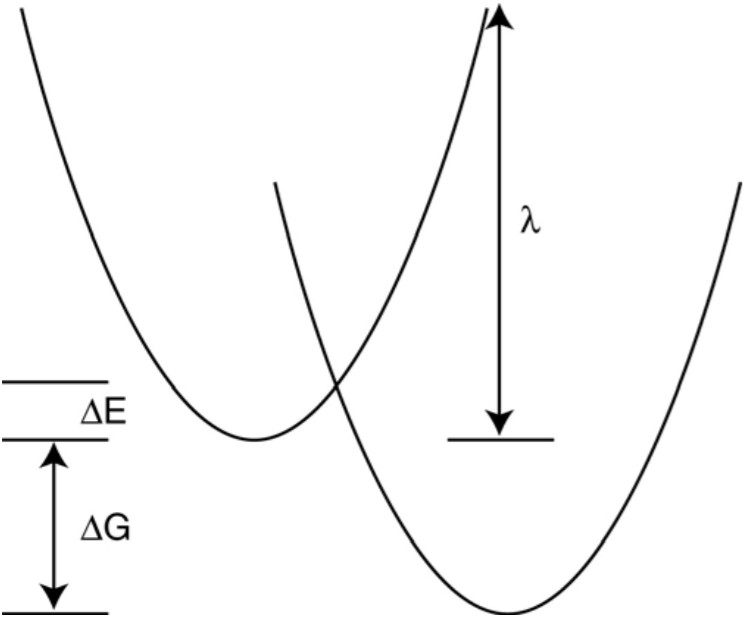
\includegraphics[scale=0.35]{marcus.jpg}
    \end{center}

    \subsection*{Mechanism contribution \small{$ \cite{web:frac} $}}

    \np{To know which mechanism predominates is important to consider the state of the reagent because may or may not be protonated and this favors differents mechanism as SPLET when specie is an anion and neutral to HAT.}

    \nec{HA \rightleftharpoons H^+ + A^- \label{8}}

    \np{For disociation reaction of monoprotic acids \eqref{8} the equation of fraction mol for the species $HA$ and $A^-$ are show in \eqref{9} and \eqref{10}}

    \nec{\chi_{_{HA}}=\frac{[H^+]}{[H^+]+k_a} \label{9}}

    \nec{\chi_{_{A^-}}=\frac{k_a}{[H^+]+k_a}\label{10}}

    \np{Hydrogen abstraction reactions from phenolic compounds are important because are antioxidant, and know information about the mechanism used to inhibit radicals are very essential to learn more.}

    \np{To know which mechanism are predominant in these reaction, we model the reaction of phenol with Hydroxyphenylradica and model by HAT \eqref{11} and SET \eqref{12}.}

    \nec{C_6H_5OH + \cdot OOH \rightarrow C_6H_5O\cdot + HOOH \label{11}}

    \nec{C_6H_5O^- + \cdot OOH \rightarrow C_6H_5O\cdot + HOO^- \label{12}}

    \section*{Materials and methods}

    \np{The modeling of the systems $C_6H_5OH$, $C_6H_5O\cdot$, $C_6H_5O^-$ , transition state $(TS)$, $HOOH$ and $HOO\cdot$ were performed with gaussView these are show in Figures 1-5.}

    \np{The calculations were performed with a laptop with an i7-8750H processor with 8GB of RAM.}

    % START FIGURE %
    \begin{figure}[h!]
      \captionsetup{justification=centering}
        % Reactive %
        \centering
        \begin{minipage}[b]{0.225\textwidth}
            \centering
          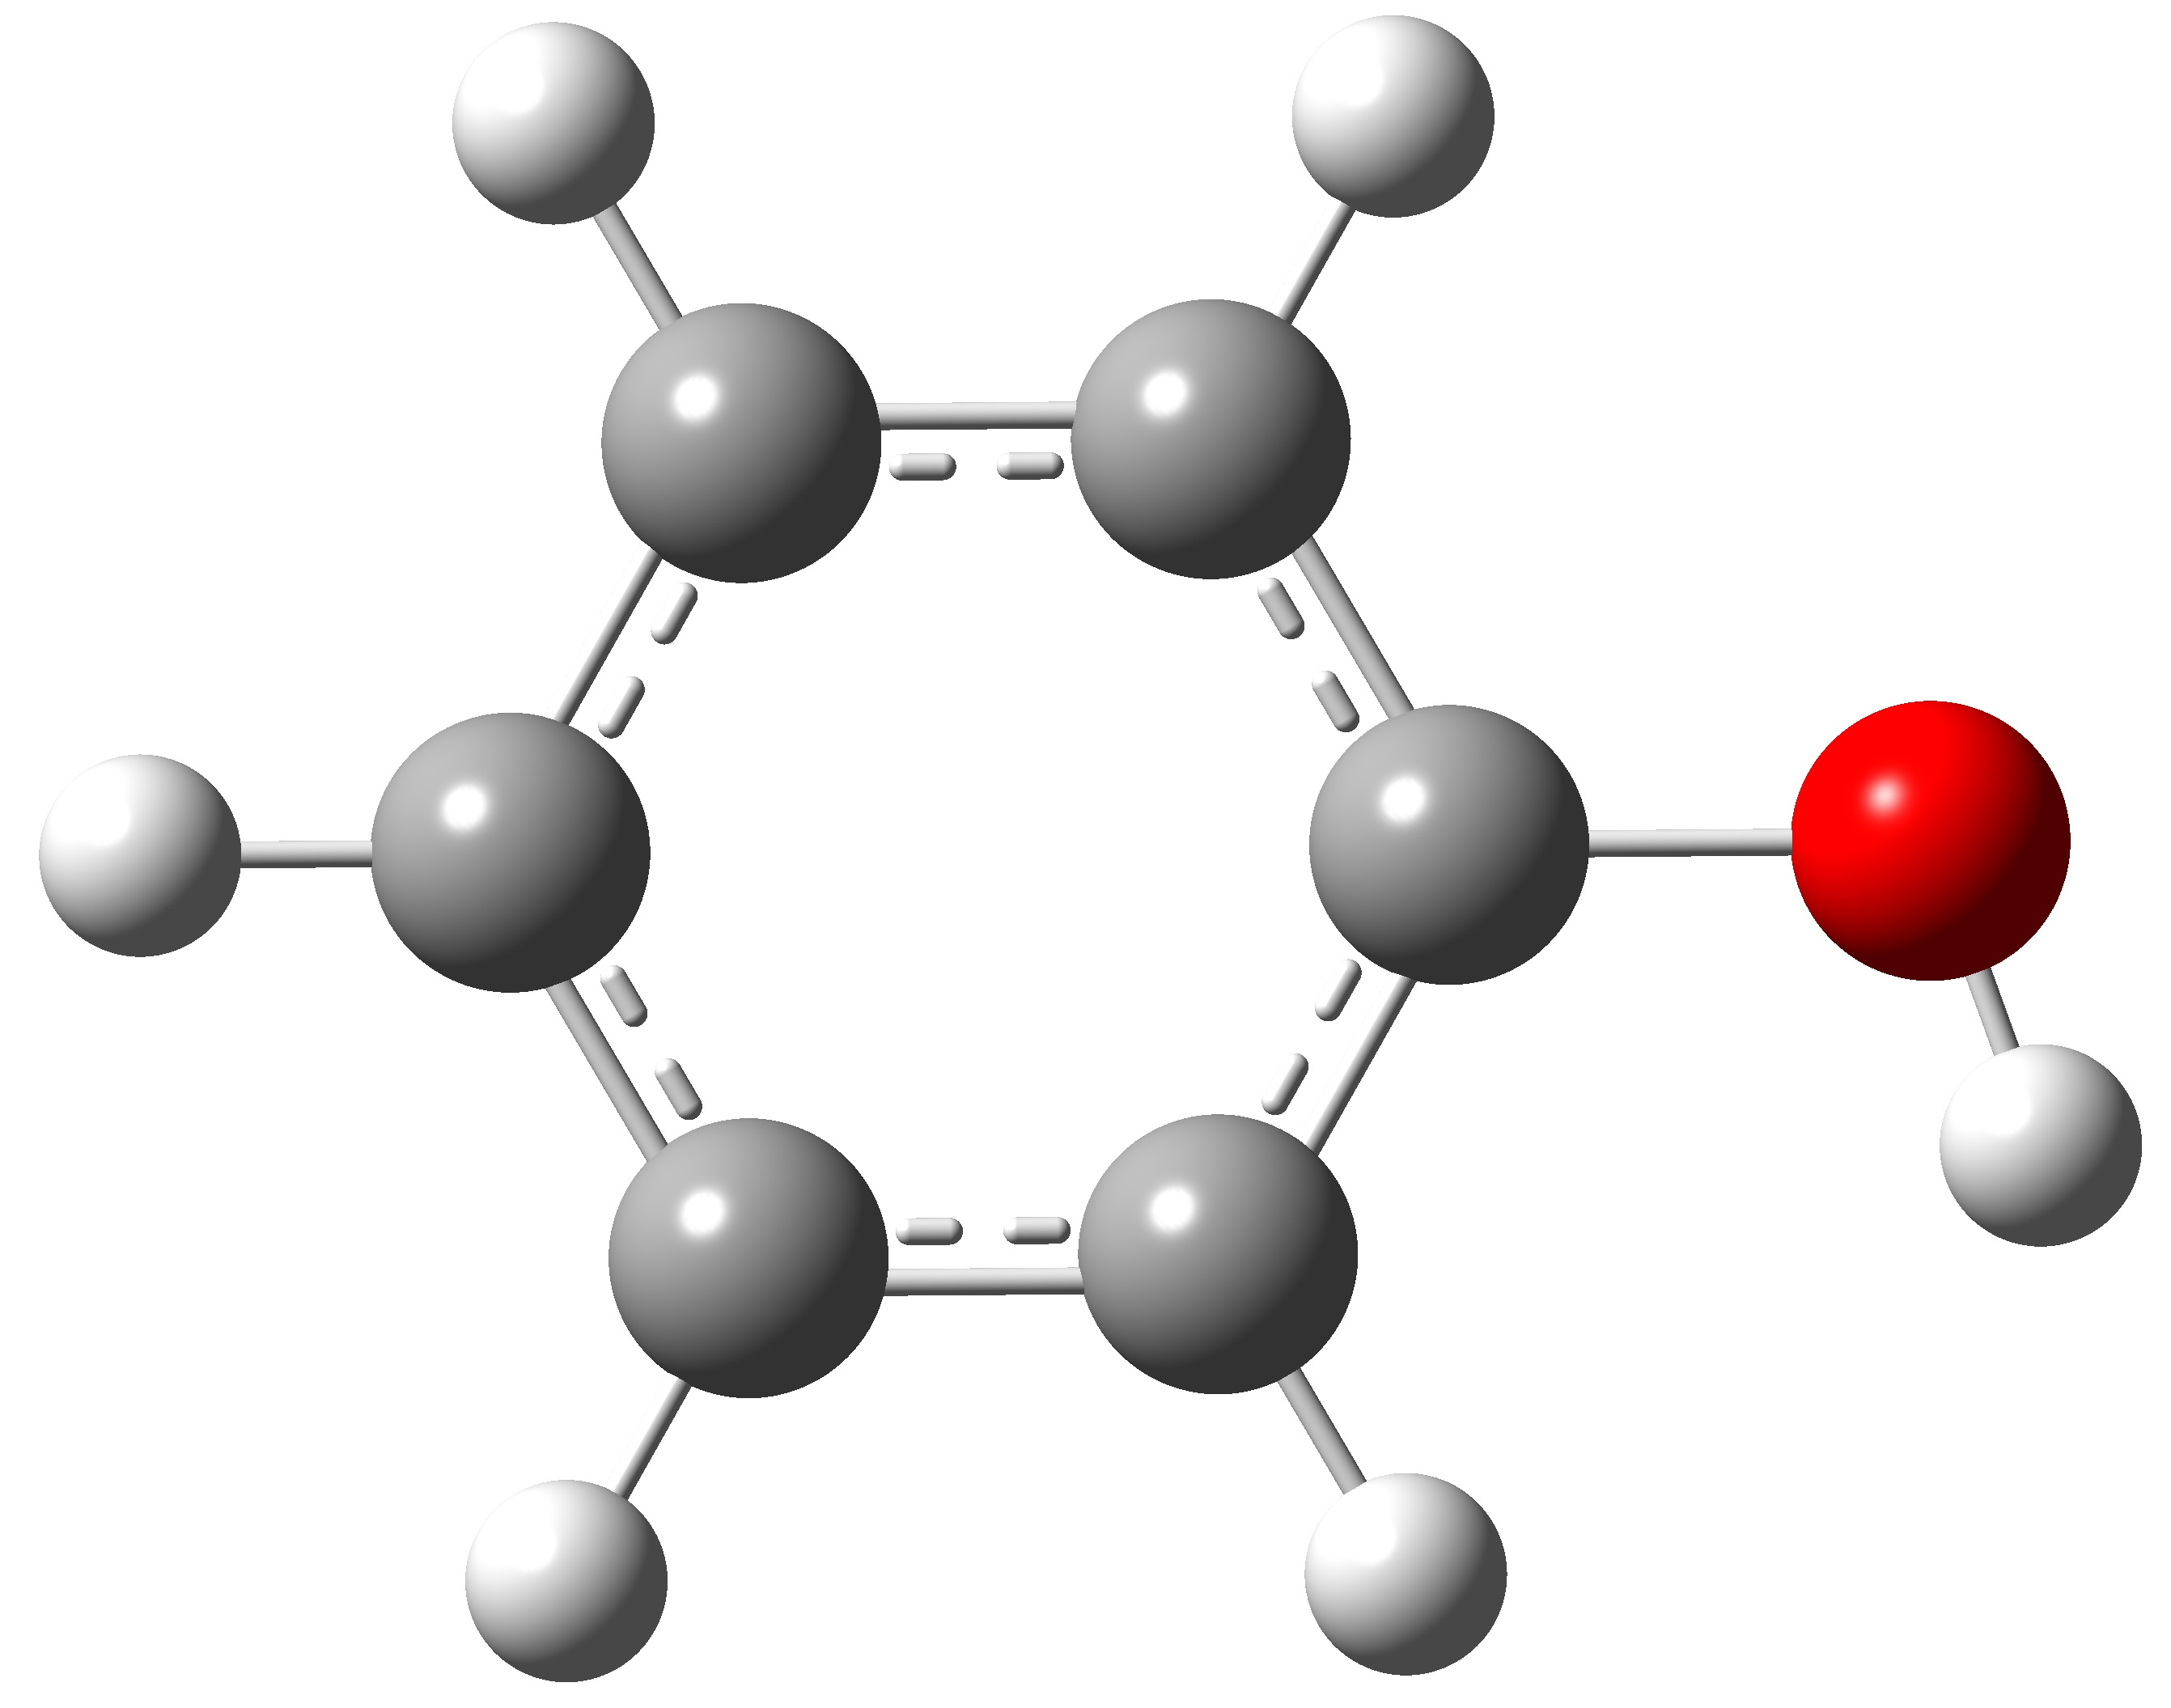
\includegraphics[scale=0.09]{fenol.jpg}
          \caption{Phenol.}
        \end{minipage}
        \hfill
        \begin{minipage}[b]{0.225\textwidth}
          \centering
          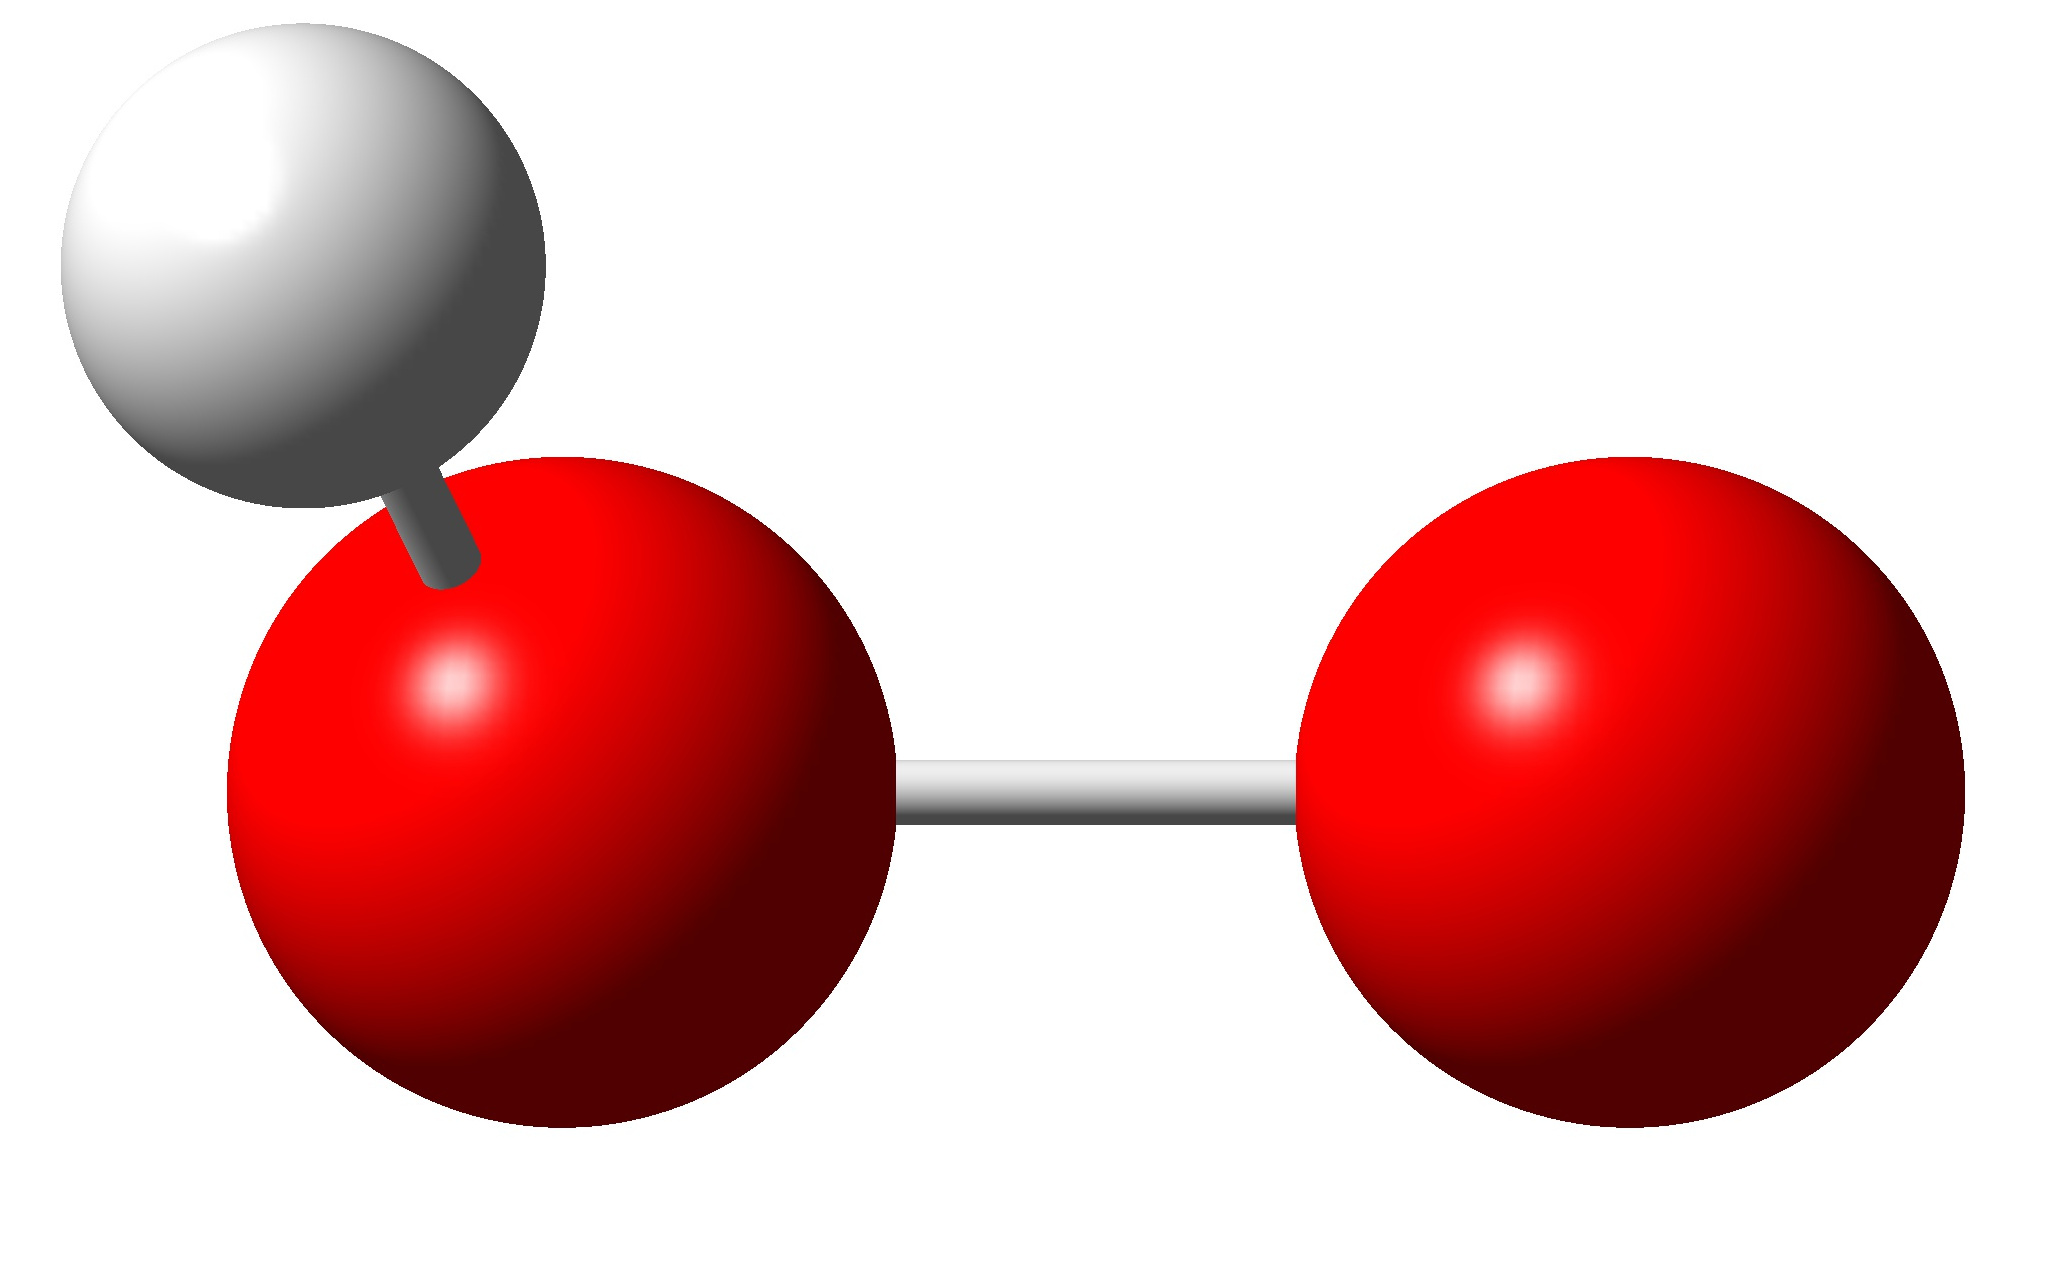
\includegraphics[scale=0.075]{hydroperoxylRadical.jpg}
          \caption{Hydroperoxyl radical/anion.}
        \end{minipage}
        %water%
        \centering
        \begin{minipage}[b]{0.45\textwidth}
            \centering
          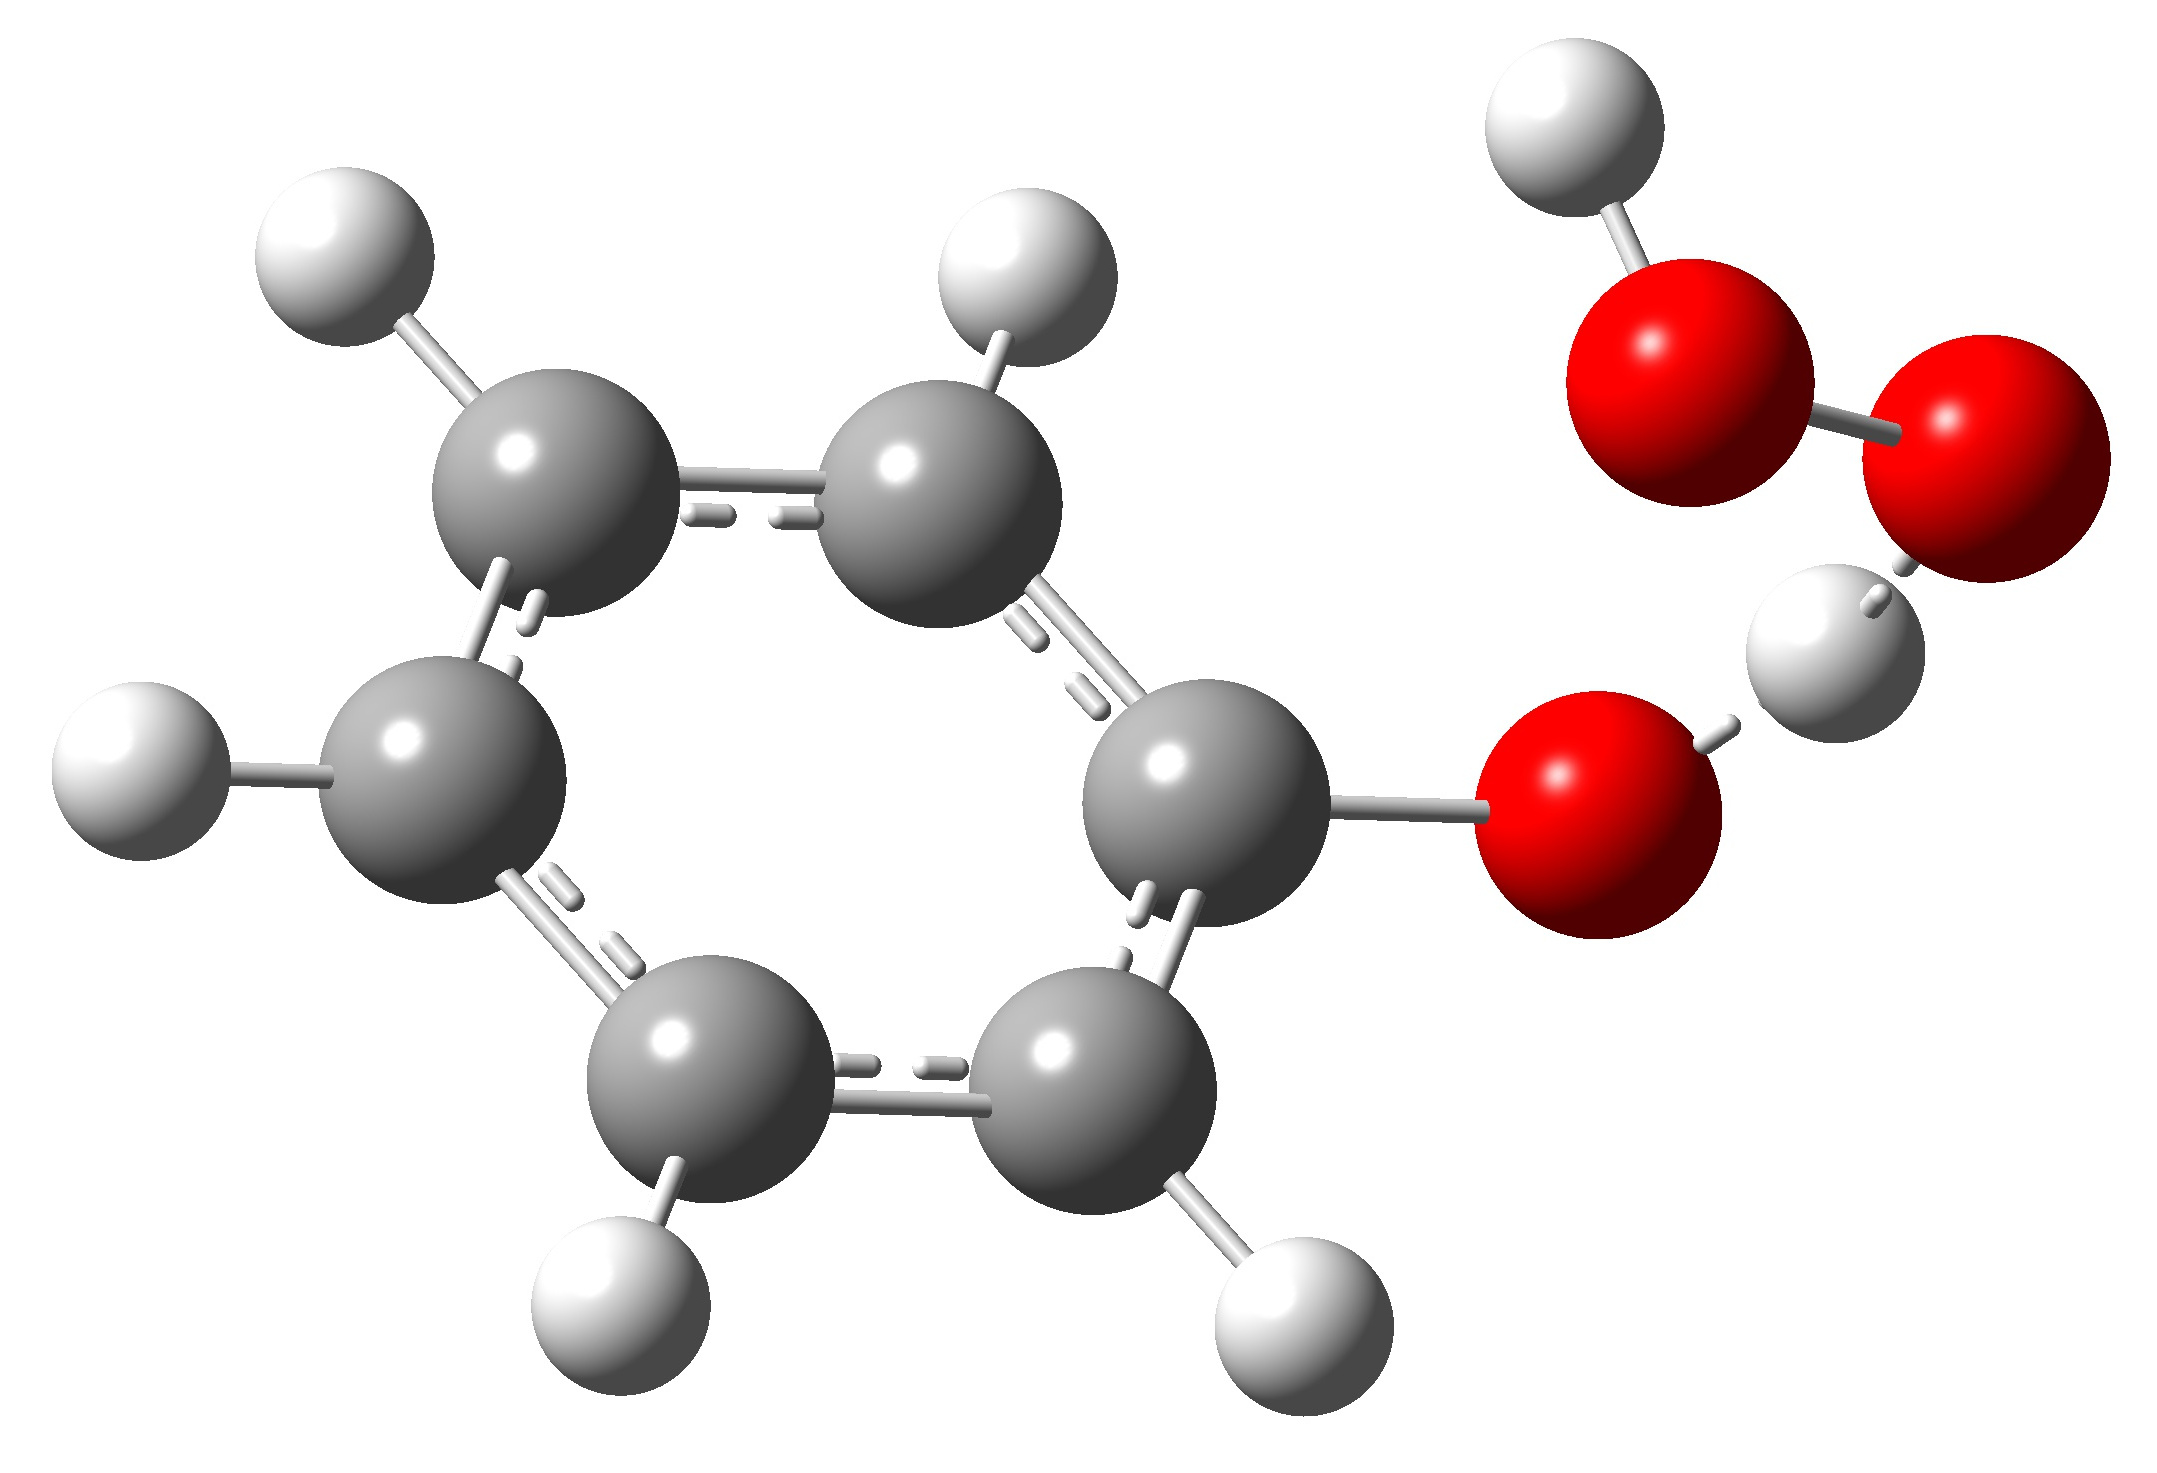
\includegraphics[scale=0.15]{ts.jpg}
          \caption{Transition state.}
        \end{minipage}
        \hfill
        \begin{minipage}[b]{0.225\textwidth}
          \centering
          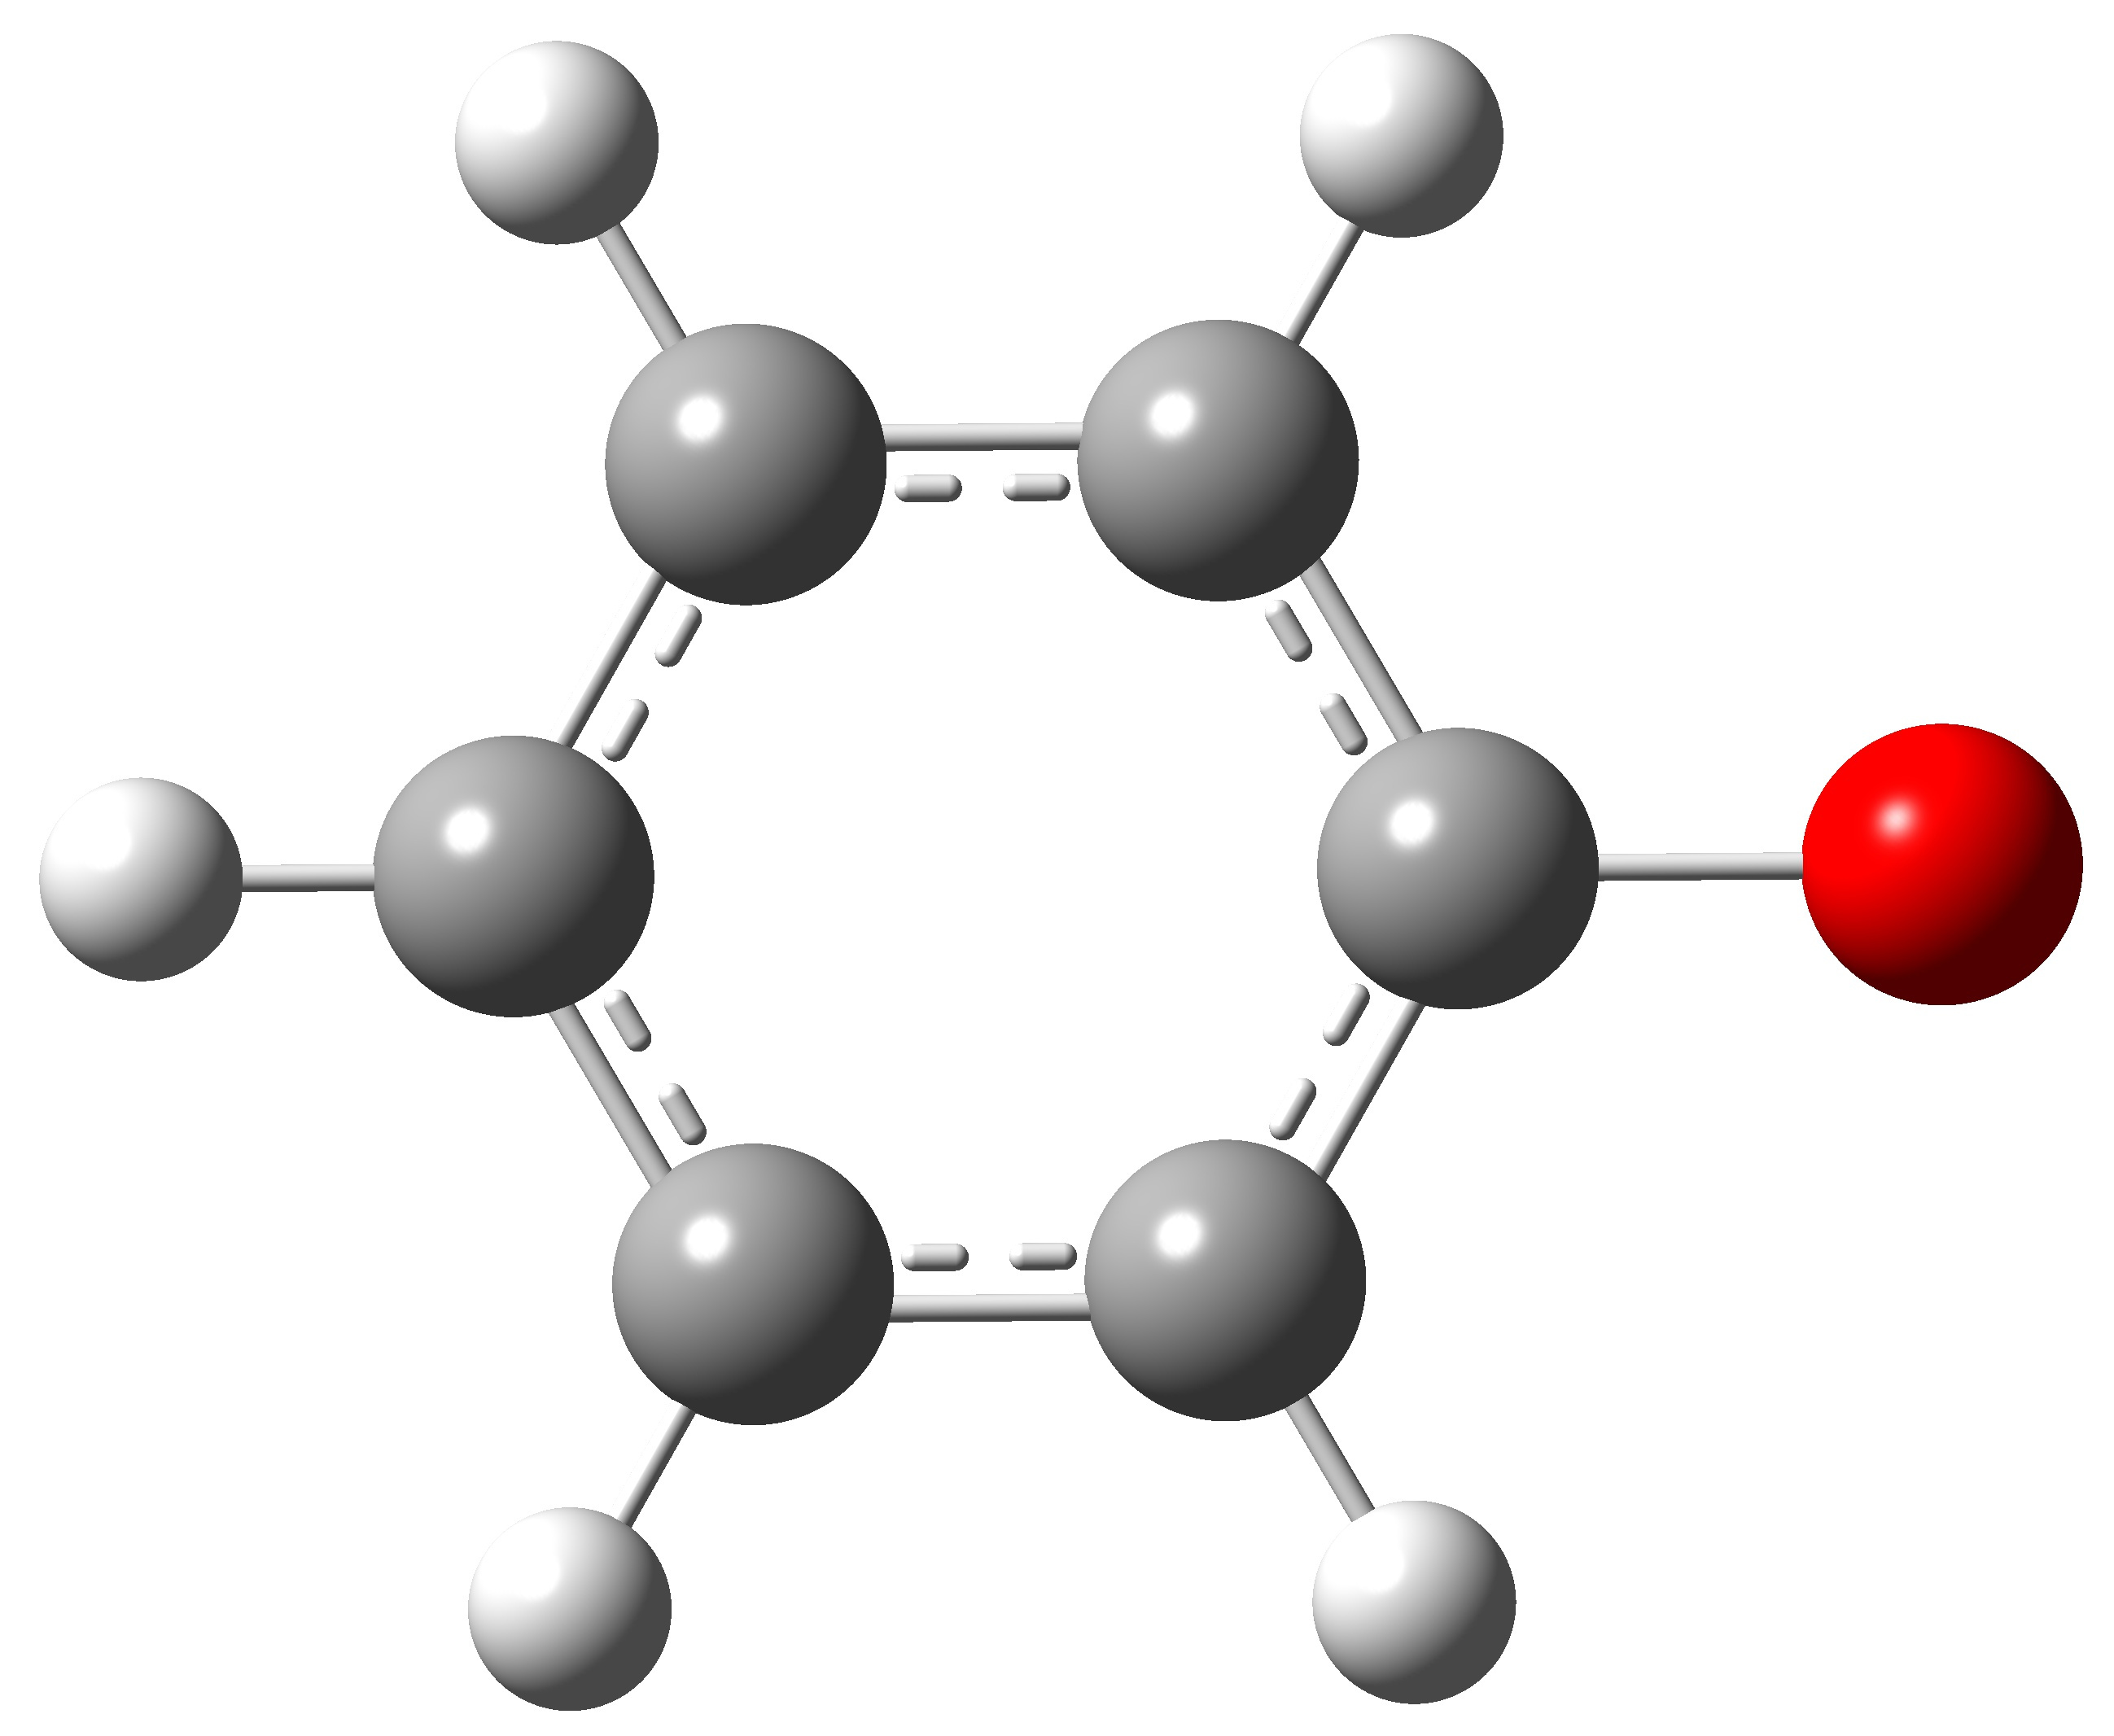
\includegraphics[scale=0.09]{hydroxyphenylRradical.jpg}
          \caption{Hydroxyphenyl radical/anion.}
        \end{minipage}
        \centering
        \begin{minipage}[b]{0.225\textwidth}
            \centering
          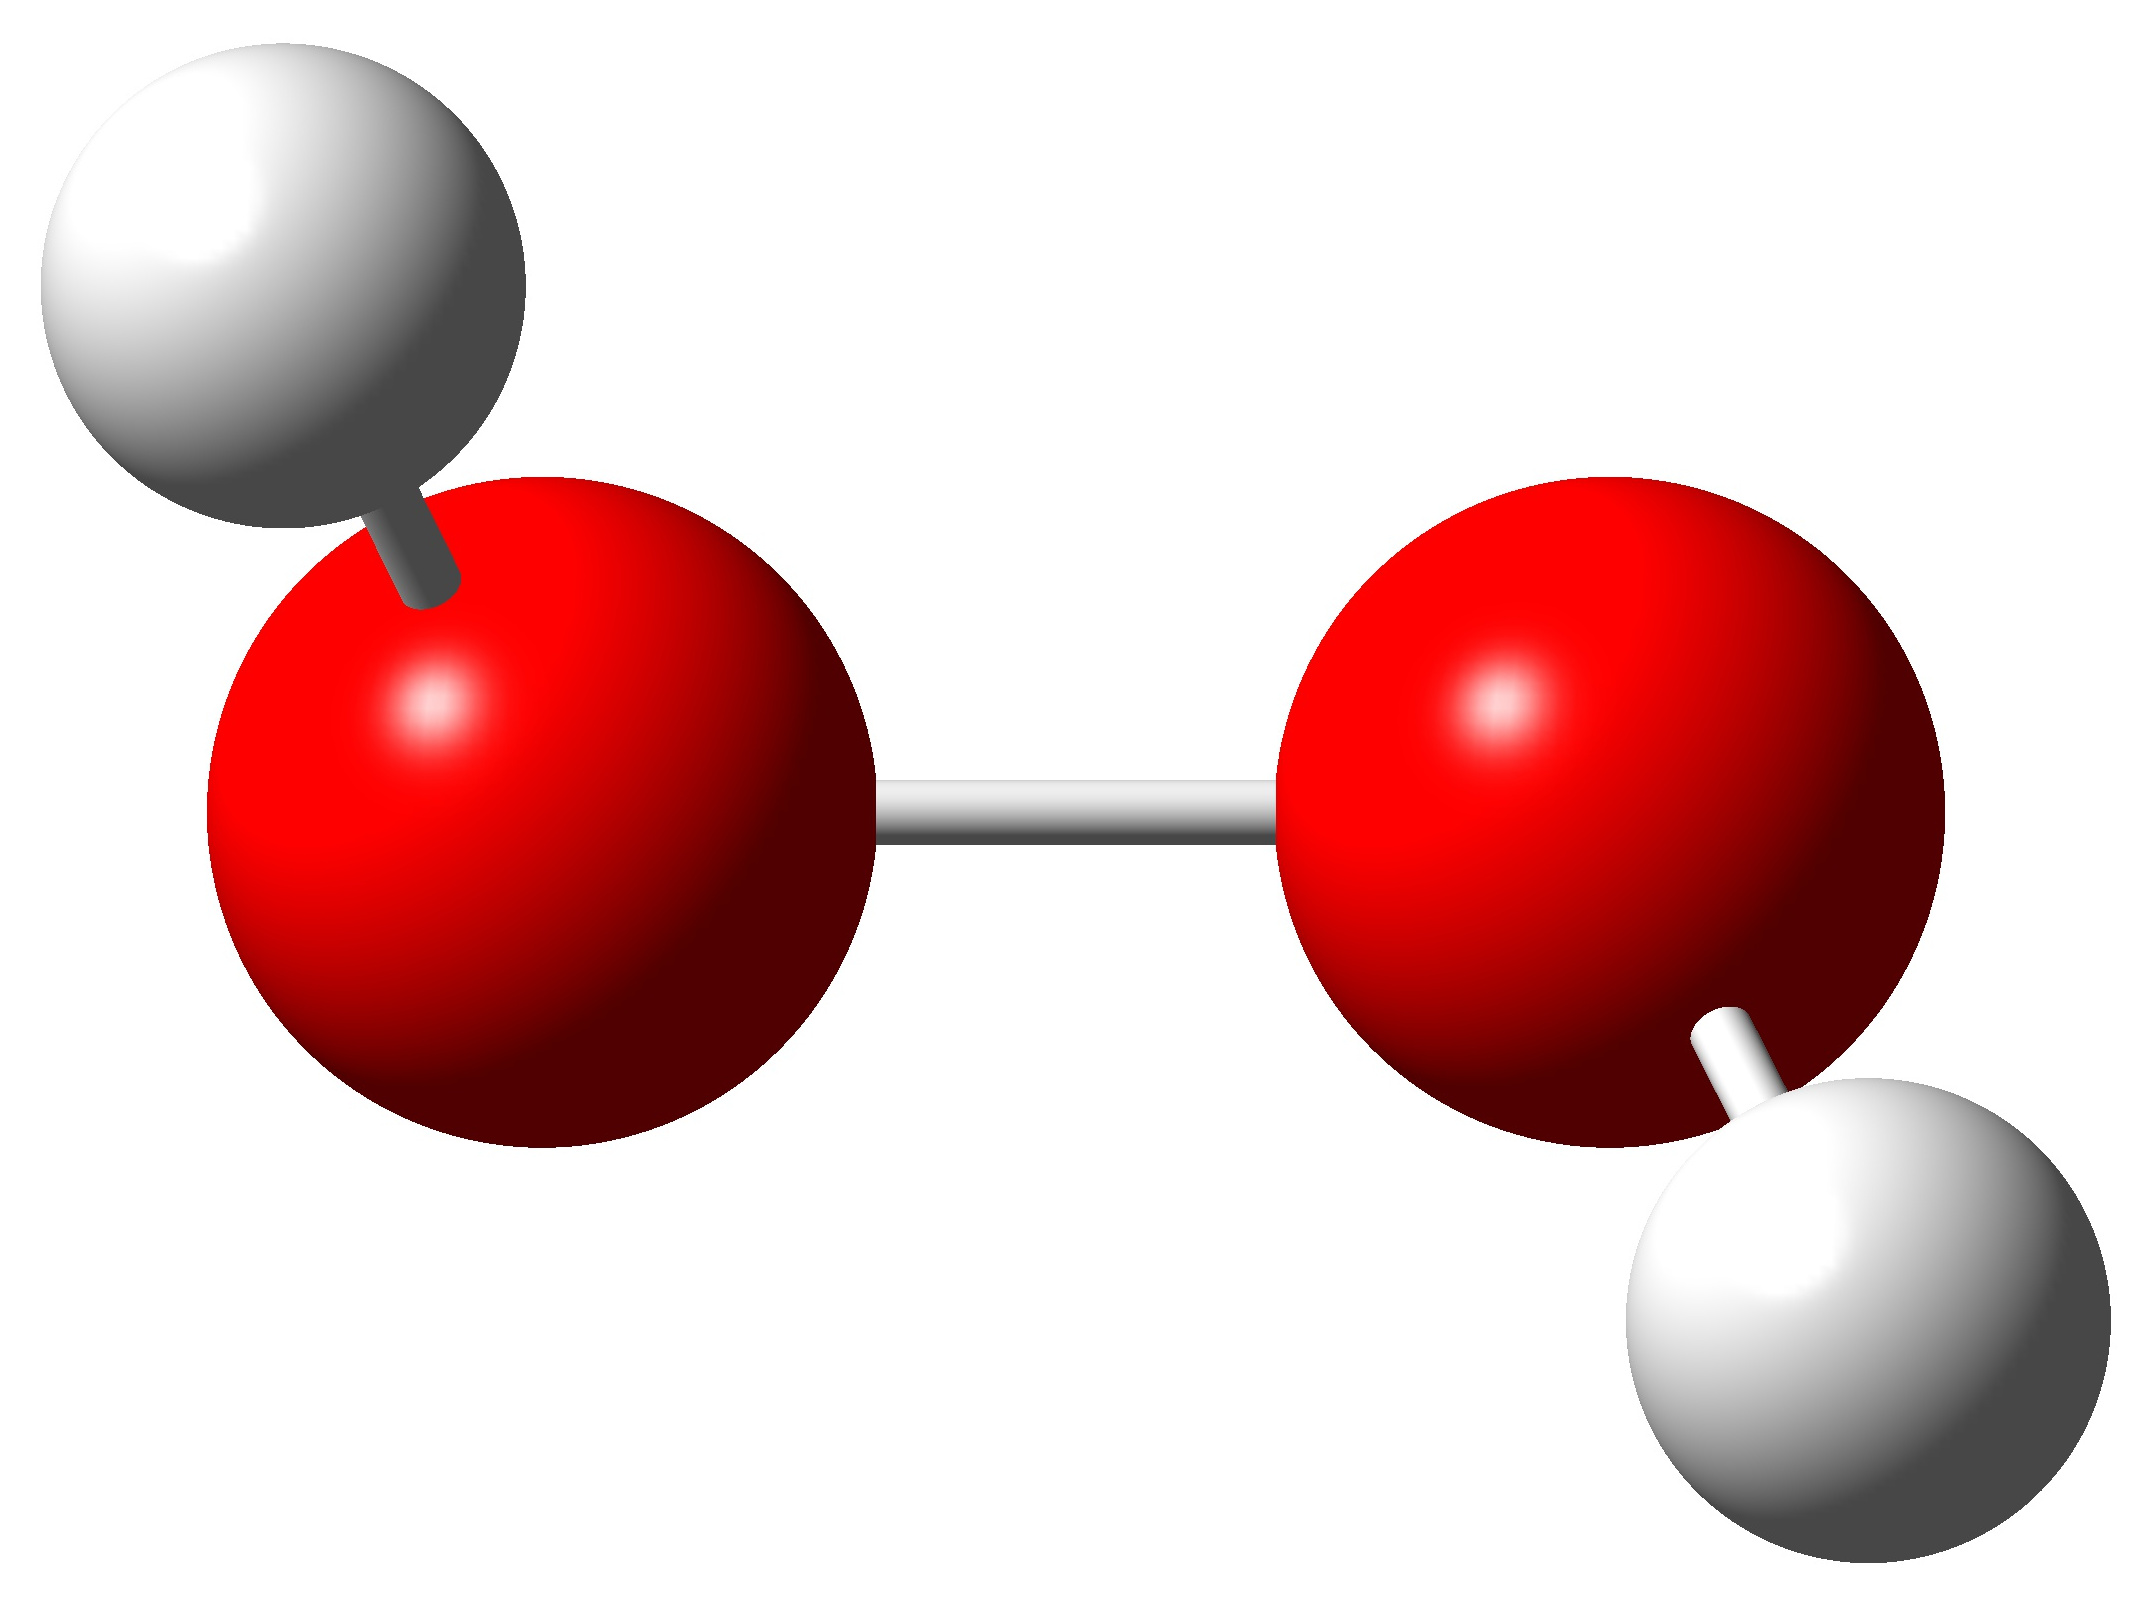
\includegraphics[scale=0.075]{hydrogenPeroxide.jpg}
          \caption{Hydrogen peroxide.}
        \end{minipage}
    \end{figure}
    % END FIGURE %

    \np{The transition state was run usign the following configuration.\n}

    \begin{lstlisting}[frame=single,gobble=10] 
            % nprocshared=4
            % mem=1500MB
            # opt(calcfc,ts,noeigen) freq=noraman 
            scrf=smd 6-31+G(d,p) iop(1/8=3) m062x
    \end{lstlisting}
    
    \np{\bt{NOTE:} The transition state was re run with the following command to converge correctly \em{\# opt(readfc,ts,noeigen) geom=check guess=check freq=noraman scrf=smd 6-31+G(d,p) iop(1/8=3) m062x}}

    \np{For reactives and products we use te following configuration.\n}

    \begin{lstlisting}[frame=single,gobble=10] 
          % nprocshared=4
          % mem=1500MB
          # opt freq scrf=smd 6-31+G(d,p) m062x
    \end{lstlisting}

    \section*{Results}

    \titleTable{1}{Values of G in Hartree for each system and Electronic energy* for systems used for SET.}

    \begin{center} 
        \item \import{./}{table1.tex}
    \end{center}

    \np{* For species used to model SET we get the value of electronic energy, in the case of the reagents we get the value of the optimization (last step of calculation which are the optimization of geometry), and the value of electronic energy of the first point of the products (which are the calculation of energy without optimization) with these are calculated the reorganization energy.}

    \np{To calculate the $\Delta G^{\ddagger}$ for SET we calculate $\lambda$, for this we calculate the $\Delta G$ and $\Delta E$ of reaction \eqref{12})}

    \np{Using the following equation.}

    \nec{(\Delta G_{prod} - \Delta G_{reac})*627.509}

    \np{Giving that $\Delta G=5.117 kcal/mol$ and $\Delta E=18.670kcal/mol$ we can calculate $\lambda$ but still, we need to make a fix, the calculation for OOH solvation is poor with only SMD so we add a correction using supermodel this is a correction of 7kcal/mol, giving a corrected value of $\Delta G=-1.882kcal/mol$ now using \eqref{7} was calculated the reorganization energy $\lambda=20.552kcal/mol$.}

    \np{Using Marcus equation \eqref{6} we get the $\Delta^{\ddagger}=4.240238719 kcal/mol$.}

    \np{Profile reaction of reaction with HAT was build with table 2.}

    \titleTable{2}{$\Delta G$ for reaction profile of HAT}

    \begin{center} 
      \item \import{./}{table2.tex}
    \end{center}
    
    \titleGraph{1}{Reaction profile for HAT}

    \begin{center}
      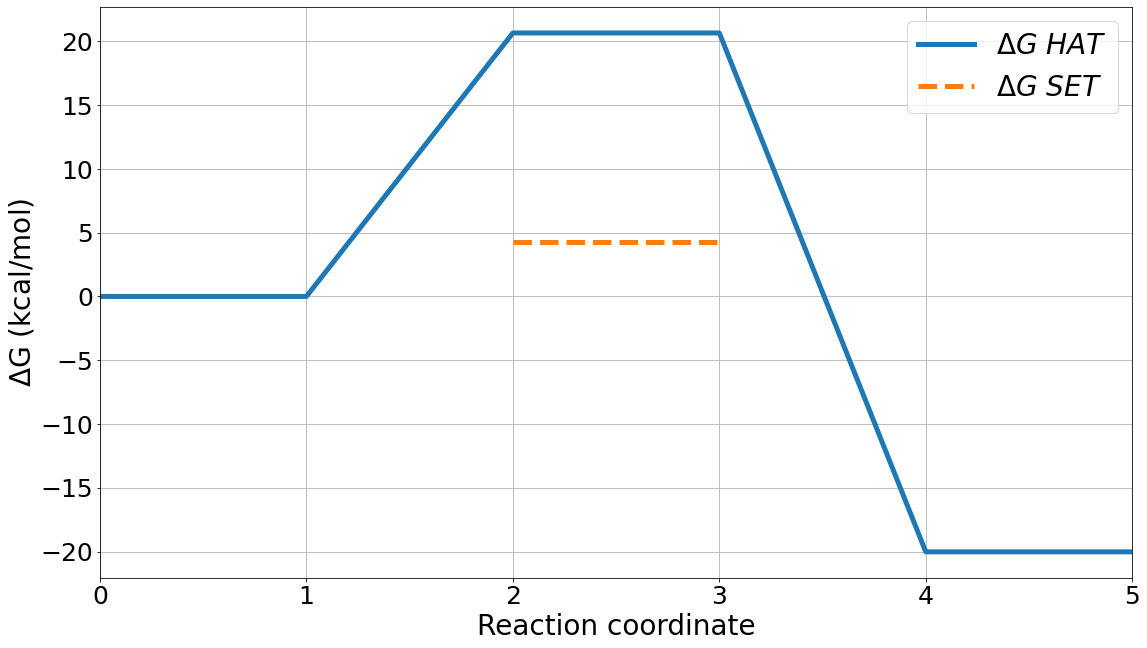
\includegraphics[scale=0.225]{profileHAT.jpg}
    \end{center}

    \np{Also using the $\Delta G^{\ddagger}$ obtained from HAT mechanism and with Eyring equation we calculated the rate constant, consider $k=1$ and $\sigma=1$, and also make a correction for standard condition 1M used by gaussian with (RT/P$\approx$ 24) and consider Benson correction ($\Delta G^{\ddagger}$-2.55 kcal/mol), for calculation of the rate constant for SET (RT/P = 1) because Marcus theory gives the correct units.}

    \np{We obtain that $K_{SET}=3.40x10^9$ and $K_{HAT}=8.02$}

    \np{Also, was considered the molar fraction of the species in physiological pH (7.4) in this pH the phenol is protonated as can be appreciated in graph 2 made with \eqref{9} and \eqref{10}.}

     \titleGraph{2}{Species distribution diagram of phenol}

    \begin{center}
      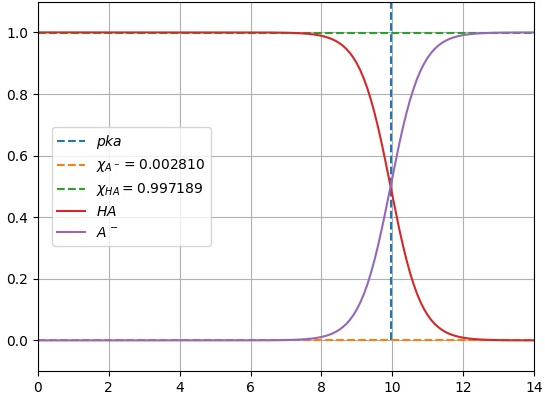
\includegraphics[scale=0.625]{./frac.jpeg}
    \end{center}

    \np{Considering the rate contant and the current fraction, and was calculate a new rate constant, $\chi_{HA}\cdot K_{HAT}=7.999$ and $\chi_{HA}\cdot K_{SET}=9.55x10^6$.}

    \section*{Discussion}

    \np{With reaction profile we can compare the activation energy of both paths, where the $\Delta G^{\ddagger}$ of SET calculated with Marcus theory show a lower barrier against the HAT, this tells us that \bt{energy required to transfer an electron is less than transfer a hydrogen atom from phenol to Hydroperoxyl radical.}}

    \np{Comparing the rate constant of both mechanisms it is very obvious the difference, where the SET rate constant is 9 orders of magnitude bigger than HAT rate constant, consider this we know that \bt{SET mechanism is faster than HAT.}}

    \np{The pH plays an important role for the predominant mechanism because SET occurs as a step of SPLET when the antioxidant is in anionic form, seeing the graph 2 we can know that in pH > pKa the mechanism predominant will be SET, but under that, we can think that predominant mechanism is HAT, but when $\chi_{A^-}$ and $\chi_{HA}$ are multiply by his rate constant, we can observe that SET rate constant is 6 orders bigger than HAT, \bt{this confirms that the predominant mechanism for the abstraction of the hydrogen atom from phenol by the hydroperoxyl radical is via SET.}}



    %% END SECTION %%
    

    %% START REFERENCES %% 




    % DEFINE STYLE FORMAT%
    \bibliographystyle{ieeetr}
    % SPECIFY THE FILE NAMEw %
    \bibliography{references}
    %% END REFERENCES %% 

    %%% THIS CONTENT IS IN TWO COLUMN (END) %%%

\end{document}
%%%%%%%%%%%%%%%% END DOCUMENT %%%%%%%%%%%%%%%%